
% syntax: none

\subsection{Dataset Plots in the Lab Color Space}\label{sec:app_labPlots}

\begin{figure}[H]
    \centering
    \foreach \i in {-1,...,33}{
      \begin{subfigure}[t]{0.146\textwidth}
        \centering       
        \ifnum \i=-1
            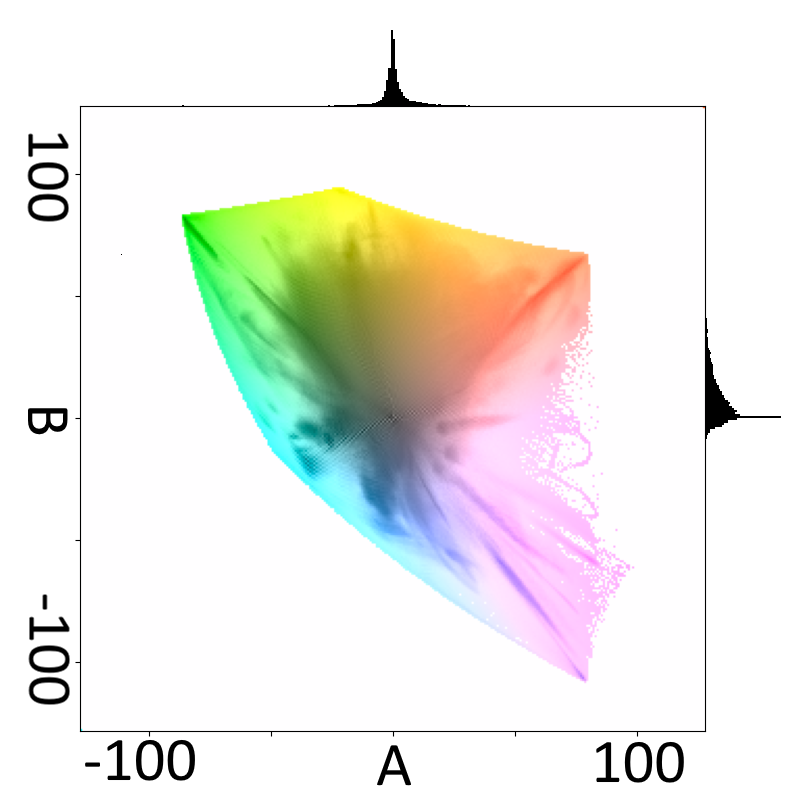
\includegraphics[width=\textwidth]{../code/dataAnalysis/plots/lab/DataCombined_lab.png}
            \caption{All Data}
        \else
            \includegraphics[width=\textwidth]{../code/dataAnalysis/plots/lab/labPlot_\i}
            \caption{source \i}
        \fi

        \label{fig:lab_sub\i}
      \end{subfigure}
      % Use the modulo operation to determine if a line break should be added
      \pgfmathparse{int(mod(\i+2,6))}
      \ifnum\pgfmathresult=0
          \newline
      \else
          \hfill
      \fi
    }
    \begin{subfigure}[t]{0.146\textwidth}
        \centering
        % No image to include, so this is left empty
        \caption*{} % Empty caption
    \end{subfigure}
    \caption{Visualization of datasets plotted in the LAB color space}
    \label{fig:lab_all}

\end{figure}

\subsection{Dataset Plots in the RGB Color Space}

\begin{figure}[H]
    \centering
    \foreach \i in {-1,...,33}{
      \begin{subfigure}[t]{0.146\textwidth}
        \centering

        \ifnum \i=-1
            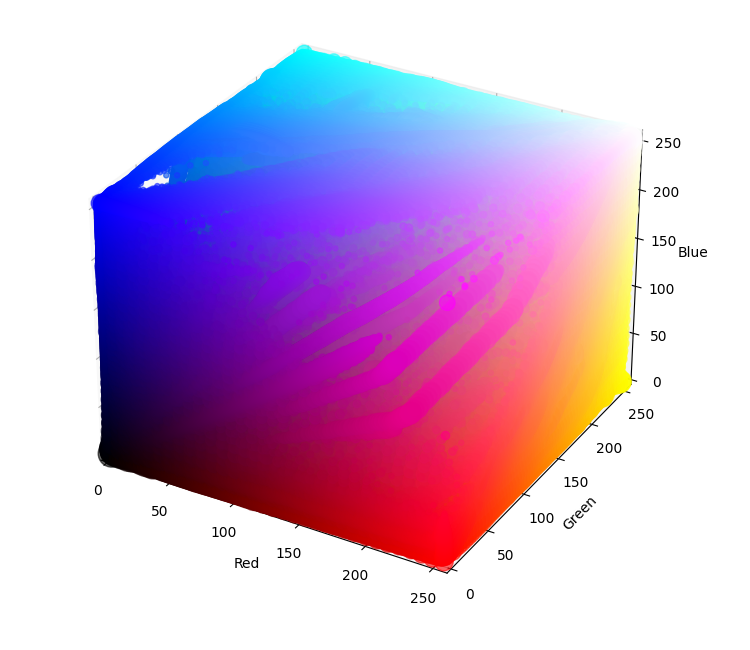
\includegraphics[width=\textwidth]{../code/dataAnalysis/plots/rgb/DataCombined_rgb.png}
        \caption{All Data}
        \else
            \includegraphics[width=\textwidth]{../code/dataAnalysis/plots/rgb/rgbPlot_\i}
            \caption{source \i}
        \fi
        \label{fig:rgb_sub\i}
      \end{subfigure}
      % Use the modulo operation to determine if a line break should be added
      \pgfmathparse{int(mod(\i+2,6))}
      \ifnum\pgfmathresult=0
          \newline
      \else
          \hfill
      \fi
    }
    \begin{subfigure}[t]{0.146\textwidth}
        \centering
        % No image to include, so this is left empty
        \caption*{} % Empty caption
    \end{subfigure}
    \caption{Visualization of datasets plotted in the RGB color space}
    \label{fig:rgb_all}
\end{figure}